\title{Assignment 2.3}
\author{
        Pradyot Prakash - 130050008
            \\
        Utkarsh Mall - 130050037
			\\
		Samarth Mishra - 130260018
}
\date{\today}
\documentclass[11pt]{article}
\usepackage[left=2.5cm,top=2cm,right=2.5cm,bottom=2cm,bindingoffset=0.5cm]{geometry}
\usepackage{graphicx}
\usepackage{siunitx}
\usepackage[section]{placeins}
\graphicspath{ {../images/} }
\renewcommand\thesubsection{\Alph{subsection}}
\begin{document}
\maketitle

Finding the $\theta$ for which the reconstuction error is minimum and using that value of  $\theta$ to reconstruct.

Minimum $\theta$ for Phantom is $105^{0}$ and for Chest CT is $53^{0}$ 

\begin{figure}[h]
\centering
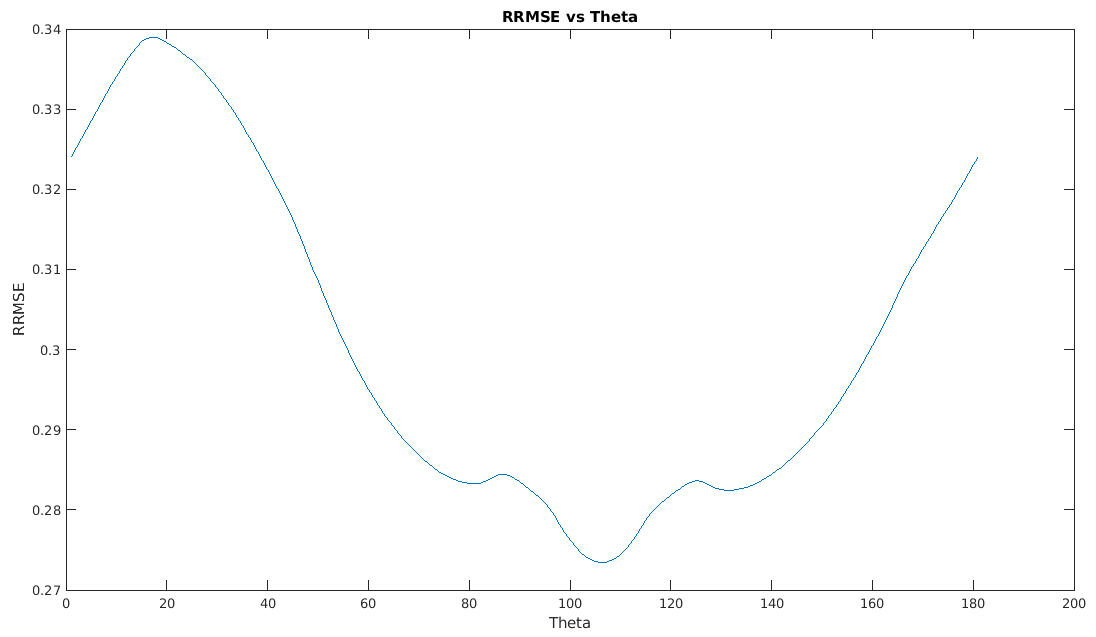
\includegraphics[scale=0.4]{phantom-plot}
\caption{RRMSE values of reconstructed image over varying $\theta$ for Phantom image}
\end{figure}
\begin{figure}[h]
\centering
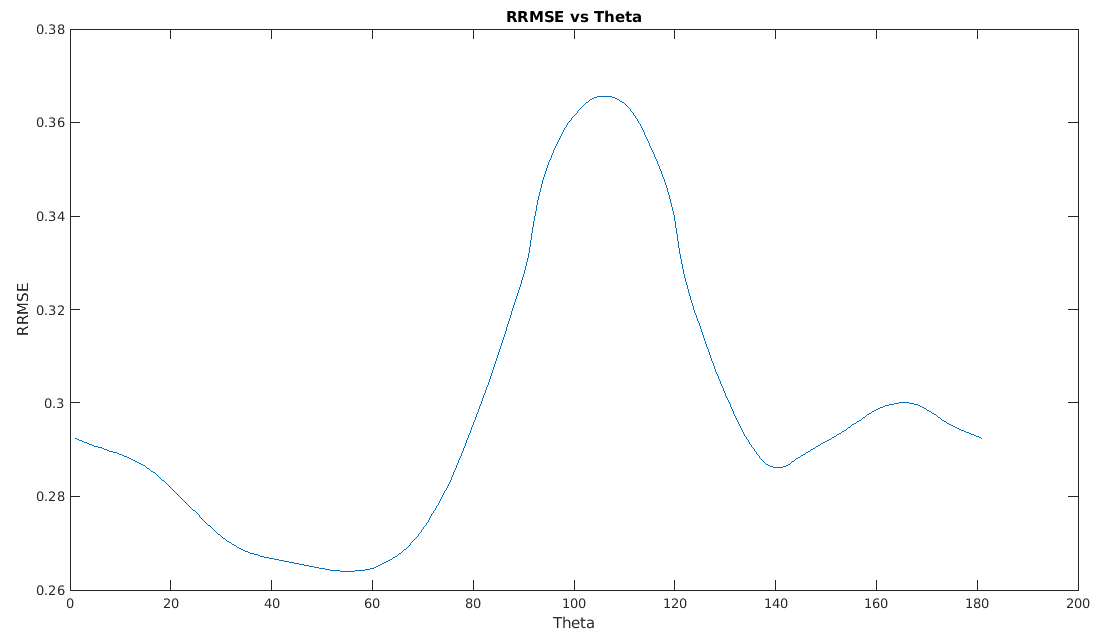
\includegraphics[scale=0.4]{CT-chest-plot}
\caption{RRMSE values of reconstructed image over varying $\theta$ for Chest CT image}
\end{figure}


\begin{figure}[h]
\centering
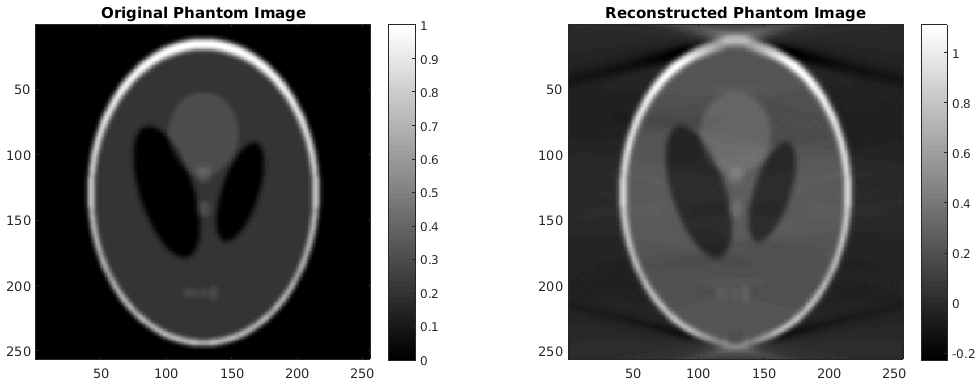
\includegraphics[scale=0.4]{phantom-recons}
\caption{Original and Reconstructed Phantom Image from partial Radon transform}
\end{figure}

\begin{figure}[h]
\centering
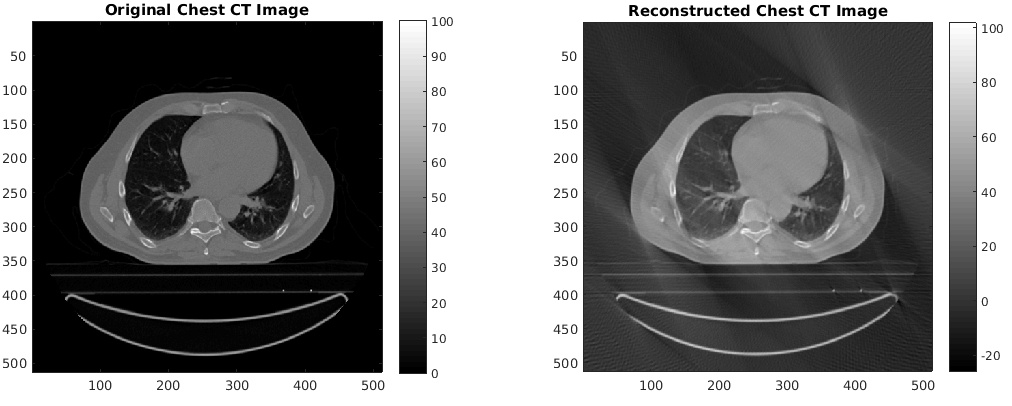
\includegraphics[scale=0.4]{CT-chest-recons}
\caption{Original and Reconstructed Chest CT Image from partial Radon transform}
\end{figure}

\end{document}
